
\documentclass{article}


\usepackage{amsfonts}
\usepackage{amsmath}
\usepackage{fancyhdr}
\usepackage{framed}
\usepackage[margin=1in]{geometry}

\pagestyle{fancy}
\fancyfoot[RE,RO]{
  \sc \footnotesize
  SMGT 435: Baseball Analytics\\
  \copyright~2024 Scott Powers}


\usepackage{tikz}
\usetikzlibrary{decorations.pathmorphing}

\begin{document}

\begin{framed}
  {\bf Caution:} These lecture notes are under construction. You may find parts that are incomplete.
\end{framed}

\setcounter{section}{5}
\section{\sc Stuff}

  Pitch outcome modeling, as presented in Chapter ??, presents a conundrum when it is used as a player evaluation tool. The most important features for predicting the outcome of a pitch are the $x$ and $z$ locations of the ball at home plate. However, these features are the least reliable when it comes to distinguishing pitchers from one another. The speed of a fastball thrown by a pitcher gives you a very good guess of the speed of the next fastball thrown by the same pitcher. But the location of a pitch thrown by a pitcher tells you very little about the location of their next pitch. To put it another way, given enough attempts, any pitcher is capable of throwing a perfectly located pitch, but very few pitchers are capable of ever throwing 100 miles per hour.

  The baseball industry has long recognized this, and pitching is often broken down into {\it Stuff} (the speed/movement of the pitch) and command/control\footnote{Control is the ability to throw strikes. Command is the ability to throw pitches in intended locations. Whether command and control are distinct skills is a topic for debate.} (the location of the pitch). Stuff encapsulates everything about the pitch trajectory except for the location of the pitch. This includes release point $(x, y, z)$, speed and movement (horizontal and vertical). The signal-to-noise ratio is very high for these features, so it takes a very small number of pitches to get an accurate estimate of a pitcher's Stuff. Command, by contrast, is much harder to evaluate.

  \subsection{\sc Observational Stuff}

    To formalize the concept of Stuff, we introduce some random variable notation.
    \begin{itemize}
      \item $Y$ represents the run value of a pitch;
      \item $X_1$ represents plate location ($x$);
      \item $X_2$ represents plate location ($z$);
      \item $X_3$ represents horizontal break;
      \item $X_4$ represents induced vertical break;
      \item $X_5$ represents pitch speed;
      \item $X_6$ represents release point ($x$);
      \item $X_7$ represents release point ($y$); and
      \item $X_8$ represents release point ($z$).
    \end{itemize}

    Using these random variables, we can write the expected run value of a pitch given its observed characteristics $x_1, ..., x_8$ as the function $f_0(\cdot)$:
    \begin{equation*}
      f_0(x_1, ..., x_8) = \mathbb{E}[Y | X_1 = x_1, ..., X_8 = x_8].
    \end{equation*}
    This function is readily estimable from the techniques discussed in the previous chapter. Recall that in Chapter ?? (Batted Ball Outcome Model), we improved the usefulness of our outcome model for batte evaluation (depending on sample size) by removing variables from the function. For pitching, the variables we remove are the $x$ and $z$ plate locations because they have the lowest signal-to-noise ratio. This leads us to our first definition of Stuff:
    \begin{equation}
      \label{eqn:observational-stuff}
      f_1(x_3, ..., x_8) = \mathbb{E}[Y | X_3 = x_3, ..., X_8 = x_8].
    \end{equation}

    This definition of Stuff has many applications in player evaluation. We can ask questions of this metric similar to the questions we have asked throughout this course. For a very small number of pitches, $f_1(\cdot)$ is a better predictor of $f_0(\cdot)$ than is $f_0(\cdot)$ itself. How many pitches does it take before $f_0(\cdot)$ becomes a better predictor of future $f_0(\cdot)$ than $f_1(\cdot)$? Because Stuff stabilizes extremely quickly, teams can use this metric to identify changes in player talent much more quickly than by using a pitch outcome model.

  \subsection{\sc Causal Stuff}

    While the definition of Stuff in the previous section (hitherto {\it observational} Stuff) is very useful for player evaluation, we prefer an alternative definition of Stuff for player development. In player evaluation, the goal is to predict player performance. In player development, the goal is to understand how changes to pitch characteristics will effect player performance. Because this is a causal question using observational data, we need to take care with how we answer it. The toy example below illustrates what can go wrong if we don't.

    \begin{center}
    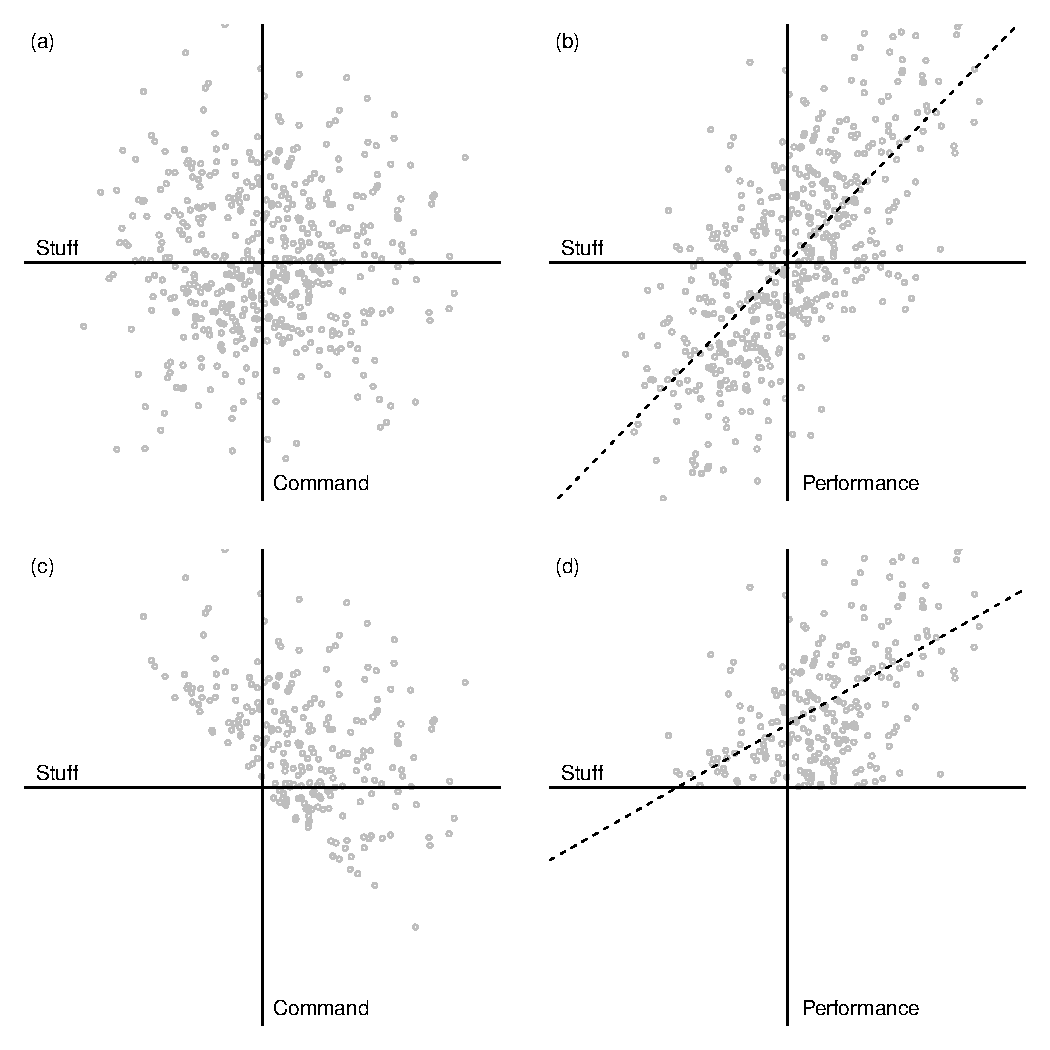
\includegraphics[width = 0.8\textwidth]{figures/stuff_selection_bias.pdf}\\
    {\it
      An illustration of how selection bias influences the observed relationship between Stuff and Performance. In this toy example, Stuff and Command are independent standard normal, and Performance = Stuff + Command. Figures (a) and (b) show the Stuff-Command and Stuff-Performance relationships in the absence of selection bias. Figures (c) and (d) show the same relationships if we only observed data for which Performance $>$ 0 (mimicking the selection of MLB pitchers). In Figure (b), the best-fit regression line is Performance = Stuff. In Figure (d), the best-fit regression line is Performance = 0.83 + 0.53 $\times$ Stuff.
    }
    \end{center}

    In the toy example, increasing a pitcher's Stuff by 1 unit (without changing their command) will increase their performance by 1 unit. However, Figure (d) shows what a linear regression would look like under selection bias. The regression shows us that a 1-unit increase in Stuff corresponds only to a 0.53-unit increase in Performance. This happens because pitchers with better Stuff tend to have worse Command (because of the selection mechanism). In the regression model, a 1-unit increase in Stuff also corresponds to a decrease in Command. Under this selection bias, the regression model fails to reveal the true relationship between Stuff and Performance.

    To fix this problem, we need to break the correlation between Stuff and command. To motivate our method, we revisit equation (\ref{eqn:observational-stuff}) and re-frame observational Stuff using the law of total expectation:
    \begin{align*}
      f_1(x_3, ..., x_8)  &= \mathbb{E}[Y | X_3 = x_3, ..., X_8 = x_8]\\
                          &= \int \int g(x_1, x_2 | x_3, ..., x_8) \mathbb{E}[Y | X_1 = x_1, ..., X_8 = x_8] dx_1 dx_2\\
                          &= \int \int g(x_1, x_2 | x_3, ..., x_8) f_0(x_1, ..., x_8) dx_1 dx_2,
    \end{align*}
    where $g(x_1, x_2 | x_3, ..., x_8)$ is the conditional probability density function of $X_1$ and $X_2$ given $X_3, ..., X_8$. In other words, we obtain Stuff by integrating expected pitch value with respect to the pitch location distribution, {\it conditional on all other characteristics}. In other words, we are averaging expected pitch value across all locations, and we are giving more weight to pitch locations more likely to co-occur with the Stuff characteristics. We can break this correlation by replacing the conditional distribution $g(x_1, x_2 | x_3, ..., x_8)$ with the marginal distribution $g(x_1, x_2)$:
    \begin{equation*}
      f_2(x_3, ..., x_8)  = \int \int g(x_1, x_2) f_0(x_1, ..., x_8) dx_1 dx_2.
    \end{equation*}
    By making this substitution, we are giving all Stuff characteristics equal opportunity to have good location (as opposed to the empirical data, where above-average Stuff characteristics are more likely to be in below-average locations). We call this second definition {\it causal} Stuff because we can use this tool to understand how a pitcher's expected pitch value will change if their Stuff characteristics change without their location quality changing.

  \subsection{\sc Discussion Questions}

    \begin{enumerate}
      \item On FanGraphs, find the current PitchingBot leaderboard (Pitching Leaderboards $\rightarrow$ Pitch Modeling). Set the minimum playing time to zero innings pitched.
      \begin{enumerate}
        \item Sort the leaderboard by botStf. How many of the top 30 players pitched at least ten innings?
        \item Sort the leaderboard by botCmd. How many of the top 30 players pitched at least ten innings?
        \item What do the results of parts (a) and (b) say about the difference between botStf and botCmd?
      \end{enumerate}
      \item Many elite pitchers have great Stuff but struggle with command. If you were a GM, would you rather develop pitchers with great command or great Stuff? Why?
      \begin{enumerate}
        \item Which do you think is easier? Developing Stuff or developing command?
      \end{enumerate}
    \end{enumerate}

\end{document}